\documentclass[letterpaper, 11pt]{article}

\usepackage{amsmath, amsthm, latexsym, amssymb, graphicx, bold-extra, mathrsfs, frcursive}
\usepackage[pdftex]{color}
\usepackage[T1]{fontenc}
\usepackage{listings}
\usepackage{adjustbox}
\usepackage{hyperref}
% Simplifies margin settings
\usepackage{geometry}
\geometry{margin=1in}

% Puts list item indicators in bold; makes flush with previous margin
\renewcommand\labelenumi{\bf\theenumi.}
\renewcommand\labelenumii{\bf\theenumii.}
% setlength\leftmargini{1.4em}
\setlength\leftmarginii{1.4em}

% Flexibility for headers and footers
\usepackage{fancyhdr}
\pagestyle{fancyplain}
\fancyhf{} %clear all header and footer fields
\lhead{\bf \small How To Write Fast Numerical Code \hspace*{\fill} Page \thepage}
\headsep 0.2in
\thispagestyle{empty}
\renewcommand{\headrulewidth}{0pt}
\renewcommand{\footrulewidth}{0pt}

\parindent 0in
\parskip 10pt
\setlength{\headheight}{20pt}

\title{ETH Zurich}

\begin{document}

%=======================================

\begin{center}
\Large \bf 263-2300-00: How To Write Fast Numerical Code

\Large \bf Assignment 4: 120 points

\large Submitted by Jinank Jain
\end{center}

\textbf{Solution 1}\\ \\
\textbf{Part a}
\begin{itemize}
\item n = 64 \\
Total number of times each element is accessed is: $3n^2$ \\
First of all lets look at the compulsory misses for matrix mat and vector v which are: 1024(=(64*64)/4) and 16(=64/4). Now lets try to calculate the conflict misses between mat and v. There is gonna be collision only with the first element of v in the inner loop and it's gonna collide only 4 times when accessing first 4 element so number of misses would be 7 (=(4*2-1)) "-1" because we already counted once initially in v one miss so we need to remove that miss.
\begin{center} Cache miss rate is $\frac{1047}{3*64*64}$ = 0.0852 \end{center}
\item n = 128 \\
Total number of times each element is accessed is: $3n^2$ \\
First lets count number of compulsory misses for matrix mat and vector v which are: 4096 (=(128*128)/4) and 32(=128/4). But in this case since whole matrix does not fit into cache unlike the previous case where whole matrix fit into cache. In this case matrix is 4 times the size of the cache. So those 7 conflict misses that we were getting in the previous case they would increase 4 times. So now total number of conflict misses are: 7*4 = 28 misses.
\begin{center}Cache miss rate is $\frac{4156}{3*128*128}$ = 0.0845 \end{center}
\end{itemize}
\textbf{Part b}
\begin{itemize}
\item n = 64 \\
Total number of times each element is accessed is: $3n^2$ \\
First of all lets count the compulsory misses in this case:
Collision would have only with vector v so we can kind remove first 16 blocks in which the whole vector v would fit in rest of the case it is just matrix mat so the compulsory misses are: 1008(=(1024-16)). \\
Now lets dig into conflict misses what happens this time since we are doing column access which would lead to a lot of conflicts. For example lets look at the first element of vector v: First we will load v[0] and then mat[0][0] and after that store v[0] back in cache so those are 3 misses. And this trend with continue for all elements of v so total number of misses are 64*3. \begin{center} Cache miss rate is $\frac{1200}{3*64*64}$ = 0.0976 \end{center}
\item n = 128 \\
Total number of times each element is accessed is: $3n^2$ \\
In this case let's first count the compulsory misses that would for matrix mat it would be 16384(=128*128) Each element would create one miss because of the column wise access to the matrix. For vector v it would 32(=128/4). \\ Now lets look at the conflicts misses with vector v and matrix mat since mat is 4 times the cache size it would conflict 4 times with each element of v so that would be 512(=128*4) \begin{center}Cache miss rate is $\frac{16928}{3*128*128}$ = 0.344 \end{center}
\end{itemize}
\bigskip

\textbf{Solution 2}
\begin{itemize}
\item Part a (n=64) \\
Total number of memory access is $\dfrac{n^2}{2}$ + n. \\
In this case if we look at the cache size which is 16KB and cache block size is 16B so number of slots in the cache would be 1024(16KB/16B).Total number of misses for vector u would be 32(=(64/4)*2) due to conflicts with vector v and total number of misses for for vector v would be 16(=64/4) and the total number of stores for matrix w would be 1024(=(64*64)/4). Thus the total number of compulsory misses are 1072.
\begin{center}Cache miss rate is $\frac{1072}{2112}$ = 0.507 \end{center}
\item Part b (n=128) \\
Total number of memory access is $\dfrac{n^2}{2}$ + n. \\
Let's first try to calculate the compulsory misses that would for u,v vector is 32(=128/4) each and matrix w it would be 4096(=(128*128)/4) and now we try to look at conflict misses that would be since matrix size is 4 times the cache size it would conflict 4 times with v so that would be 128(=32*4) and additional 8 misses for conflict between u and v.
\begin{center}Cache miss rate is $\frac{4296}{8320}$ = 0.516 \end{center}
\item Part c \\
There can be other strategy which can make the situation worse. If u and v are separated by 16KB they will collide more in cache blocks and therefore increase cache misses.  For n= 64 there will be 64 misses for u, 96 misses for v and 1024 misses for matrix mat. \begin{center}Cache miss rate is $\frac{1184}{2112}$ = 0.561 \end{center}
\end{itemize}
\bigskip

\textbf{Solution 3}\\ \\
\textbf{Part a} \\
In order to plot the roofline plot we need two parameters Bandwidth between cache and memory in byte/cycle ($\beta$) and Peak Performance($\pi$). In case of non-vectorized FMA peak performance would be 4 F/C while in the case of vectorized code peak performance would be 16 F/C. In order to calculate $\beta$ we are given that memory bandwidth is 13GB/s and frequency of the processor is 3.5 GHz so memory bandwidth in bytes/cycle would be 3.99(=13*1024/(3.5*1000)). So the roofline plot would look something like Fig. 1
\begin{figure}[h!]
	\centering
    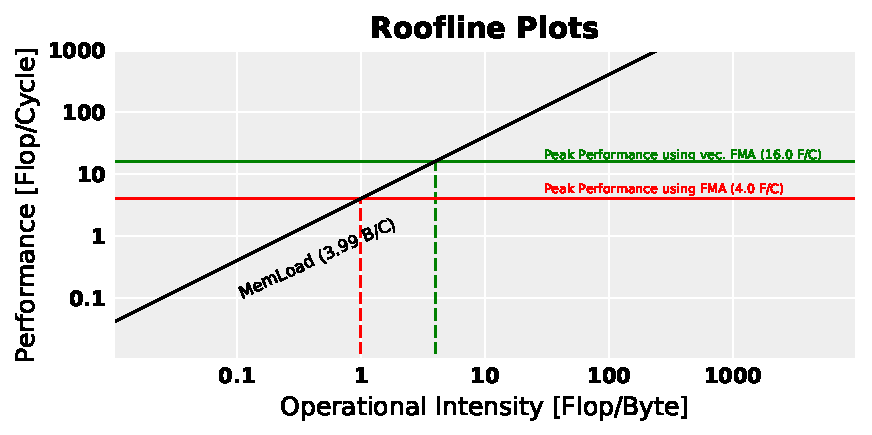
\includegraphics[width=100mm]{basic-rooflinePlot}
    \caption{Roofline plot for part a Question 3}
\end{figure}

\textbf{Part b}
\begin{figure}[h!]
	\centering
    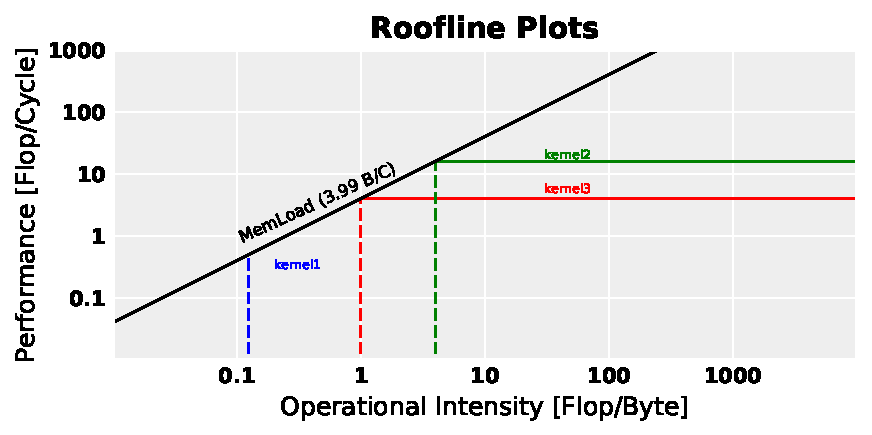
\includegraphics[width=100mm]{part2}
    \caption{Roofline plot for part b Question 3}
\end{figure}
\begin{itemize}
\item Operational Intensity
\begin{itemize}
\item kernel1 \\ \\
Total number of ops: 2$N$ \\
Total number of read-write: 2$N$*8 \\ \\
Operational Intensity: $\dfrac{1}{8}$ \\
\item kernel2 \\ \\ 
Total number of ops: 2$N^3$ \\
Total number of read-write: 4$N^2$*8 \\ \\
Operational Intensity: $\dfrac{N}{16}$\\
\item kernel3 \\ \\
Total number of ops: 4$N^3$ \\
Total number of read-write: (4$N^2$+2N)*8 \\ \\
Operational Intensity: $\dfrac{N^2}{8N+4} \approx \dfrac{N}{8} $\\
\end{itemize}
\item Maximum Theoretical Performance
\begin{itemize}
\item kernel1 \\ \\
We cannot reach max performance of 16 F/C because our code is memory bounded looking at the operation intensity. Maximum performance that we would be able to reach would be 0.498 F/C
\item kernel2 \\ \\
Maximum performance that you can reach is 16 F/C with vectorized code and we can reach the maximum performance since our complete working set fits in cache. But whether we would reach that max. performance or not depends on the value of N.
\begin{center}
if N $\geq$ 64, perf = 16 F/C \\
else performance is bounded by memory bandwidth and it follow the slanted line.
\end{center}
\item kernel3 \\ \\
Maximum performance that you can reach is 4 F/C with non vectorized code and we can reach the maximum performance since our complete working set fits in cache. But whether we would reach that max. performance or not depends on the value of N.
\begin{center}
if N $\geq$ 8, perf = 4 F/C \\
else performance is bounded by memory bandwidth and it follow the slanted line.
\end{center}
\end{itemize}
\end{itemize}

\textbf{Part c} \\ 
One common observation would be we would bit right in the graph as operational intensity would increase as we move from doubles to floats as we can perform more ops and less data.
\begin{figure}[h!]
	\centering
    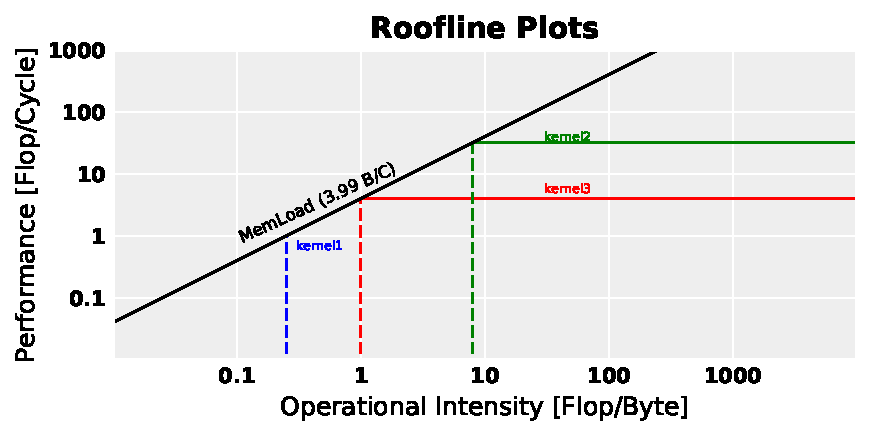
\includegraphics[width=100mm]{part3}
    \caption{Roofline plot for part c Question 3}
\end{figure}
\begin{itemize}
\item Operational Intensity
\begin{itemize}
\item kernel1 \\ \\
Total number of ops: 2$N$ \\
Total number of read-write: 2$N$*4 \\ \\
Operational Intensity: $\dfrac{1}{4}$ \\
\item kernel2 \\ \\ 
Total number of ops: 2$N^3$ \\
Total number of read-write: 4$N^2$*4 \\ \\
Operational Intensity: $\dfrac{N}{8}$\\
\item kernel3 \\ \\
Total number of ops: 4$N^3$ \\
Total number of read-write: (4$N^2$+2N)*4 \\ \\
Operational Intensity: $\dfrac{N^2}{4N+2} \approx \dfrac{N}{4} $\\
\end{itemize}
\item Maximum Theoretical Performance
\begin{itemize}
\item kernel1 \\ \\
We cannot reach max performance of 32 F/C because our code is memory bounded looking at the operation intensity. Maximum performance that we would be able to reach would be 0.9975 F/C.
\item kernel2 \\ \\
Maximum performance that you can reach is 32 F/C with vectorized code because we can fit 4 floats in place 2 doubles so our peak performance has increased and we can reach the maximum performance since our complete working set fits in cache. But whether we would reach that max. performance or not depends on the value of N.
\begin{center}
if N $\geq$ 64, perf = 32 F/C \\
else performance is bounded by memory bandwidth and it follow the slanted line.
\end{center}
\item kernel3 \\ \\
Maximum performance that you can reach is 4 F/C with non vectorized code and we can reach the maximum performance since our complete working set fits in cache. But whether we would reach that max. performance or not depends on the value of N.
\begin{center}
if N $\geq$ 4, perf = 4 F/C \\
else performance is bounded by memory bandwidth and it follow the slanted line.
\end{center}
\end{itemize}
\end{itemize}

\bigskip

\clearpage

%=======================================

\end{document}